% 10_appendix_floats.tex -- tables and figures for this section (2026-10-15), each \input from a generated/ file or an
% \includegraphics of a generated figure; generators: writeup/make_rehaul_*.py. Placed after the section in paper_rehaul.tex
% so section text and floats can be edited in parallel; move them inline when the prose settles.
%
% Generator: writeup/make_rehaul_appendix.py -> generated/rehaul_app_*.tex (tables) and generated/rehaul_app_numbers.tex
% (\rhapp... macros: every number in the captions and notes below). Re-run it after any source changes:
%   python writeup/make_rehaul_appendix.py
% Order: A1 tree tuning rungs; A2 MinGRU development; A3 robustness figures; A4 the all-features MinGRU diagnosis.
% Each group ends with \clearpage so the float queue never overflows.
\ifdefined\rhappNdays\else% AUTO-GENERATED by writeup/make_rehaul_appendix.py -- do not edit.
% Source: every number quoted in rehaul/10_appendix_floats.tex and rehaul/08_feature_importance_floats.tex captions
\newcommand{\rhappNdays}{866}
\newcommand{\rhappNblocks}{5}
\newcommand{\rhappAllbarsRinitAll}{0.2298}
\newcommand{\rhappAllbarsRinitBase}{0.2358}
\newcommand{\rhappAllbarsWdBAll}{0.2630}
\newcommand{\rhappAllbarsWdBBase}{0.2480}
\newcommand{\rhappNvariants}{35}
\newcommand{\rhappNmonthEnd}{43}
\newcommand{\rhappNextreme}{60}
\newcommand{\rhappNother}{763}
\newcommand{\rhappNmonthEndExtreme}{5}
\newcommand{\rhappExtremeCols}{10}
\newcommand{\rhappGapShareExtreme}{71}
\newcommand{\rhappGapShareMonthEnd}{60}
\newcommand{\rhappGapShareOther}{\ensuremath{-}31}
\newcommand{\rhappNcolsBase}{22}
\newcommand{\rhappNcolsAll}{628}
\newcommand{\rhappNsessionEdge}{12}
\newcommand{\rhappNsessionEdgeHalf}{6}
\newcommand{\rhappOptExch}{20}
\newcommand{\rhappOptTrials}{50}
\newcommand{\rhappOptPoints}{1{,}469}
\newcommand{\rhappShiftNfc}{9}
\newcommand{\rhappShiftNdays}{865}
\newcommand{\rhappShiftKmin}{\ensuremath{-}12}
\newcommand{\rhappShiftKmax}{6}
\newcommand{\rhappShiftNnot}{85}
\newcommand{\rhappMurphyNc}{33}
\newcommand{\rhappModelSetN}{94}
\newcommand{\rhappModelSetPaper}{9}
\newcommand{\rhappModelSetPooledLin}{6}
\newcommand{\rhappModelSetPerBarLin}{7}
\newcommand{\rhappModelSetPerBarTrees}{72}
\newcommand{\rhappCompF}{3}
\newcommand{\rhappCompDays}{614}
\newcommand{\rhappFiRefits}{147}
\newcommand{\rhappFiSeries}{49}
\newcommand{\rhappFiClusters}{166}
\newcommand{\rhappFiColsEligible}{564}
\newcommand{\rhappFiBootBlock}{6}
\newcommand{\rhappFiDraws}{10}
\newcommand{\rhappFiClusterCorr}{0.8}
\newcommand{\rhappFiRefitEvery}{10}
\newcommand{\rhappFiTimeTop}{5}
\newcommand{\rhappFiTimeSmooth}{5}
\newcommand{\rhappFiTimeCap}{20}
\newcommand{\rhappFiConstCols}{137}
\fi
% 2026-10-15 (notation pass): \fqsDMLag / \fqsHACLag (Newey-West lags) are used in the notes below.
\ifdefined\fqsPairs\else% AUTO-GENERATED by writeup/make_fig_qlike_sharpe.py -- do not edit.
% Figure writeup/figures/fig_qlike_sharpe.pdf: QLIKE against Sharpe (mid), HAR + calendar vs all
% features, every model of results/close_master_table/paper_model_set.csv on both input sets
% (per-bar linear = the pre-tuned subpt_* rows; LSTMs excluded); numbers from master_table.csv
% and master_table_daily.parquet.  Changes are all features minus HAR + calendar, on the same days.
% DM: dm_test on the daily QLIKE difference; t: hac_inference.llsw_test on the daily mid-return
% difference (614 post-warmup days, bandwidth 33, fixed-b p); Sharpe changes: Ledoit-Wolf p;
% ES(c = 1): close_murphy_splits_headline.elementary on f / iv, y / iv.  Point estimates.
% pooled pairs: family pooled twin
\newcommand{\fqsPairs}{42}  % models on both input sets (pairs drawn)
\newcommand{\fqsPairsPerBarLinear}{3}  % of which per-bar linear (pre-tuned)
\newcommand{\fqsPairsPooled}{3}  % of which pooled 48-bar linear
\newcommand{\fqsPairsTree}{36}  % of which per-bar trees
\newcommand{\fqsPoints}{85}  % points drawn: both ends of every pair + the HAR + cal. OLS
\newcommand{\fqsDays}{866}  % trade days
\newcommand{\fqsQLower}{31}  % QLIKE lower with all features
\newcommand{\fqsQLowerSig}{3}  % ... and DM significant at 5 %
\newcommand{\fqsQHigher}{11}  % QLIKE higher with all features
\newcommand{\fqsQHigherSig}{0}  % ... and DM significant at 5 %
\newcommand{\fqsQLowerSigLagFourteen}{2}  % sensitivity: QLIKE lower, DM at lag 14 significant
\newcommand{\fqsQHigherSigLagFourteen}{0}  % sensitivity: QLIKE higher, DM at lag 14 significant
\newcommand{\fqsShHigher}{41}  % Sharpe (mid) higher with all features
\newcommand{\fqsShHigherSig}{6}  % ... and Ledoit-Wolf p < 0.05 (614 post-warmup days)
\newcommand{\fqsShLower}{1}  % Sharpe (mid) lower with all features
\newcommand{\fqsShLowerSig}{0}  % ... and Ledoit-Wolf p < 0.05 (614 post-warmup days)
\newcommand{\fqsQLowerShHigher}{30}  % both: QLIKE lower and Sharpe higher
\newcommand{\fqsMedDQ}{\ensuremath{-}0.0016}  % median QLIKE change (all features minus HAR + cal.)
\newcommand{\fqsMedDQPct}{\ensuremath{-}1.6}  % median QLIKE change, % of the HAR + cal. QLIKE
\newcommand{\fqsMedDSh}{\ensuremath{+}0.53}  % median Sharpe (mid) change
\newcommand{\fqsESLower}{29}  % elementary score at the threshold (c = 1) lower with all features
\newcommand{\fqsCorrES}{0.07}  % Pearson corr. across pairs: ES(c = 1) change vs HAC t of the P&L change
\newcommand{\fqsCorrQ}{0.12}  % Pearson corr. across pairs: QLIKE change vs HAC t of the P&L change
\newcommand{\fqsInShade}{4}  % all-features points in the shaded quadrant
\newcommand{\fqsInShadeBase}{3}  % HAR + cal. points in the shaded quadrant
\newcommand{\fqsOlsQ}{0.0967}  % QLIKE of the HAR + cal. OLS
\newcommand{\fqsOlsSh}{1.06}  % Sharpe (mid) of the HAR + cal. OLS
\newcommand{\fqsDMLag}{6}  % Newey-West lag of the DM statistic (the master table's)
\newcommand{\fqsHACS}{33}  % bandwidth S of the t of the mean P&L change (LLSW 2018, 614 post-warmup days)
\newcommand{\fqsSigPct}{5}  % two-sided level of the counts, %
\newcommand{\fqsQuadBetterBoth}{30}  % change figure: lower QLIKE, higher Sharpe
\newcommand{\fqsQuadShOnly}{11}  % change figure: higher QLIKE, higher Sharpe
\newcommand{\fqsQuadQOnly}{1}  % change figure: lower QLIKE, lower Sharpe
\newcommand{\fqsQuadWorseBoth}{0}  % change figure: higher QLIKE, lower Sharpe
\fi

% =====================================================================================================================
% A1. Tree tuning rungs. The tables re-lay out the campaign's generated tables (numbers copied verbatim by the
% generator, which parses them): generated/table_close_ladder.tex (make_table_close_main.py) and
% generated/appendix_campaign_16h_{cadence,mask,tuneper,budget,budget_oos,optuna_vs,picks}.tex
% (make_appendix_campaign_16h_tex.py). The originals overflow the text width at \small (by 5--190 pt), hence the re-layout.
% =====================================================================================================================

% Source: generated/table_close_ladder.tex
\begin{table}[htbp]
\centering
\small
\setlength{\tabcolsep}{3.5pt}
\begin{threeparttable}
% 2026-10-15 (notation pass): parked -- code jargon (16:00 ladder, per-bar, rungs)
% \caption{The 16:00 ladder: one change at a time, from the paper's forecast to the per-bar specification and through
% the tree rungs.}
% 2026-10-15 (table legibility): short caption, details in the notes; notes cut to about five sentences, method
% details referred to Methods. The pre-notation-pass caption and notes are parked in the comments here.
\caption{Decomposition of the closing-interval results}
\label{tab:rh_app_tune_ladder}
% AUTO-GENERATED by writeup/make_rehaul_appendix.py -- do not edit.
% Source: writeup/generated/table_close_ladder.tex (numbers verbatim; its sources are listed there)
\begin{tabular}{@{}l*{6}{r}@{}}
\toprule
 & \multicolumn{2}{c}{QLIKE} & \multicolumn{3}{c}{Sharpe ratio} & Same \\
\cmidrule(lr){2-3}\cmidrule(lr){4-6}
Step (to minus from) & $\Delta$\% & DM & $\Delta$, mid & HAC $t$ & $\Delta$, crossed & side (\%) \\
\midrule
\multicolumn{7}{@{}l}{\emph{From the paper's forecast to the per-bar specification}} \\
\quad block-diag.\ ridge $\to$ pooled ridge, all features & \ensuremath{-}4.3 & \ensuremath{-}1.75 & +0.16 & +0.34 & +0.16 & 88 \\
\addlinespace
\multicolumn{7}{@{}l}{\emph{Fit the 16:00 bar alone: pooled twin $\to$ per-bar ridge}} \\
\quad HAR + calendar & \ensuremath{-}11.3 & \ensuremath{-}3.42 & +0.46 & +1.05 & +0.46 & 88 \\
\quad all features & \ensuremath{-}6.2 & \ensuremath{-}1.56 & \ensuremath{-}0.03 & \ensuremath{-}0.07 & \ensuremath{-}0.02 & 86 \\
\addlinespace
\multicolumn{7}{@{}l}{\emph{Inputs of the per-bar ridge}} \\
\quad HAR + calendar $\to$ all features & +1.2 & +0.26 & +0.05 & +0.09 & +0.04 & 86 \\
\addlinespace
\multicolumn{7}{@{}l}{\emph{Estimator on all features: per-bar ridge $\to$ alternative}} \\
\quad lasso & \ensuremath{-}4.5 & \ensuremath{-}1.60 & +0.46 & +1.28 & +0.47 & 92 \\
\quad elastic net & \ensuremath{-}1.6 & \ensuremath{-}1.04 & +0.50 & +1.59 & +0.50 & 93 \\
\quad LightGBM, shipped, refit every 10 & +0.5 & +0.14 & \ensuremath{-}0.05 & \ensuremath{-}0.13 & \ensuremath{-}0.05 & 85 \\
\quad XGBoost, shipped, refit every 10 & +1.3 & +0.37 & +0.13 & +0.35 & +0.13 & 85 \\
\quad random forest, shipped, refit every 10 & +2.5 & +0.56 & \ensuremath{-}0.15 & \ensuremath{-}0.34 & \ensuremath{-}0.13 & 85 \\
\quad LightGBM, random search, refit every 10 & +2.5 & +0.56 & +0.39 & +0.93 & +0.40 & 85 \\
\quad XGBoost, random search, refit every 10 & +5.1 & +1.14 & +0.26 & +0.46 & +0.26 & 84 \\
\quad random forest, random search, refit every 10 & +10.6 & +1.85 & \ensuremath{-}0.30 & \ensuremath{-}0.81 & \ensuremath{-}0.29 & 86 \\
\addlinespace
\multicolumn{7}{@{}l}{\emph{Campaign, design: the 12 session-edge duplicates dropped}} \\
\quad per-bar ridge, one penalty (campaign's) & +0.0 & --- & +0.00 & --- & +0.00 & 100 \\
\addlinespace
\multicolumn{7}{@{}l}{\emph{Campaign, per-window mask: masked minus unmasked}} \\
\quad LightGBM, shipped, refit every 10 & \ensuremath{-}1.0 & \ensuremath{-}1.01 & \ensuremath{-}0.21 & \ensuremath{-}0.69 & \ensuremath{-}0.21 & 96 \\
\quad LightGBM, shipped, refit daily & +1.4 & +1.39 & \ensuremath{-}0.23 & \ensuremath{-}0.55 & \ensuremath{-}0.23 & 94 \\
\quad LightGBM, random search, refit every 10 & +2.6 & +1.34 & \ensuremath{-}0.08 & \ensuremath{-}0.32 & \ensuremath{-}0.08 & 94 \\
\quad LightGBM, random search, refit daily & +0.1 & +0.03 & \ensuremath{-}0.05 & \ensuremath{-}0.17 & \ensuremath{-}0.05 & 94 \\
\addlinespace
\multicolumn{7}{@{}l}{\emph{Campaign, refit cadence: every 10 sessions $\to$ every session}} \\
\quad LightGBM, shipped settings & \ensuremath{-}2.4 & \ensuremath{-}1.23 & \ensuremath{-}0.04 & \ensuremath{-}0.08 & \ensuremath{-}0.04 & 93 \\
\addlinespace
\multicolumn{7}{@{}l}{\emph{Campaign, tuning (LightGBM, refit daily)}} \\
\quad shipped settings $\to$ random search & +2.9 & +1.05 & +0.28 & +0.58 & +0.28 & 91 \\
\quad shipped settings $\to$ Optuna, tuned daily & +7.5 & +2.87 & \ensuremath{-}0.10 & \ensuremath{-}0.31 & \ensuremath{-}0.10 & 91 \\
\quad Optuna: tuned every 250 sessions $\to$ daily & +2.8 & +0.81 & \ensuremath{-}0.32 & \ensuremath{-}0.65 & \ensuremath{-}0.33 & 90 \\
\bottomrule
\end{tabular}

\begin{tablenotes}[flushleft]
\footnotesize
% 2026-10-15 (notation pass): parked -- code jargon (paired step, trade days, sign(s), crossed fill, shipped settings, config ids); test wording
% \item[] \emph{Notes:} each row is a paired step, to minus from, over \rhappNdays{} trade days; point estimates.
% QLIKE $\Delta$\%: $100\,(\mathrm{QLIKE}_{\text{to}}/\mathrm{QLIKE}_{\text{from}} - 1)$. DM: Diebold--Mariano statistic
% of the daily QLIKE difference (---: not stored for that pair). Sharpe $\Delta$: change in the annualised $\sign(s)$
% Sharpe ratio at the mid and crossed fills. HAC $t$: Newey--West $t$ of the daily mid-return difference. Same side:
% share of days on which the two forecasts take the same position. Shipped settings: LightGBM \texttt{lgbm\_opt\_00},
% XGBoost \texttt{xgb\_opt\_00}, random forest trial 255, the top entries of the 1998--2002 development searches.
\item[] \textit{Notes:} Each row compares two forecasts (``to'' minus ``from''), one change at a time, from the earlier
draft's pooled intraday forecast to the closing-interval specification and through the tuning specifications of the
tree models, over the \rhappNdays{} trading days of the out-of-sample period; point estimates. QLIKE $\Delta$\%:
$100\,(\overline{\QLIKE}_{\text{to}}/\overline{\QLIKE}_{\text{from}} - 1)$; $\DM$: Diebold--Mariano statistic of the
daily QLIKE loss differential, with the Harvey--Leybourne--Newbold correction and Newey--West lag $q = \fqsDMLag$
(---: not stored). Sharpe ratio $\Delta$: change in the annualized Sharpe ratio of the sign strategy at mid-quotes and
at quoted bid--ask prices; HAC $t$: HAC $t$-statistic on the daily return differential at mid-quotes (Newey--West,
$q = \fqsHACLag$). Same side: share of trading days on which the two forecasts take the same position. Fixed
hyperparameters and tuning procedures: see Methods (\emph{Tuning procedures}).
% Fixed hyperparameters = LightGBM lgbm_opt_00, XGBoost xgb_opt_00, random forest trial 255.
\end{tablenotes}
\end{threeparttable}
\end{table}

% Source: generated/appendix_campaign_16h_cadence.tex
\begin{table}[htbp]
\centering
\small
\begin{threeparttable}
% 2026-10-15 (notation pass): parked -- code jargon (refit cadence, input set)
% \caption{Refit cadence and random search, by tree and input set.}
% 2026-10-15 (table legibility): short caption, details in the notes; notes cut to about five sentences, method
% details referred to Methods. The pre-notation-pass caption and notes are parked in the comments here.
\caption{Re-estimation frequency and random search}
\label{tab:rh_app_tune_cadence}
% AUTO-GENERATED by writeup/make_rehaul_appendix.py -- do not edit.
% Source: writeup/generated/appendix_campaign_16h_cadence.tex (numbers verbatim; its sources are listed there)
\begin{tabular}{@{}l*{6}{r}@{}}
\toprule
 & \multicolumn{2}{c}{T1 $-$ T10} & \multicolumn{2}{c}{RS1 $-$ RS10} & \multicolumn{2}{c}{RS1 $-$ T1} \\
\cmidrule(lr){2-3}\cmidrule(lr){4-5}\cmidrule(lr){6-7}
Model & QLIKE & $\Delta$SR & QLIKE & $\Delta$SR & QLIKE & $\Delta$SR \\
\midrule
\multicolumn{7}{@{}l}{\emph{HAR + calendar}} \\
\quad LightGBM & \ensuremath{-}0.8 & \ensuremath{+}0.06 & \ensuremath{+}0.2 & \ensuremath{-}0.31 & \ensuremath{+}5.9 & \ensuremath{-}0.15 \\
\quad XGBoost & \ensuremath{+}0.1 & \ensuremath{-}0.25 & \ensuremath{-}0.2 & \ensuremath{-}0.42 & \ensuremath{+}9.3 & \ensuremath{-}0.38 \\
\quad Random forest & \ensuremath{-}1.5 & \ensuremath{-}0.31 & \ensuremath{+}0.1 & \ensuremath{+}0.03 & \ensuremath{+}9.4 & \ensuremath{+}0.01 \\
\addlinespace
\multicolumn{7}{@{}l}{\emph{All features}} \\
\quad LightGBM & \ensuremath{-}2.4 & \ensuremath{-}0.04 & \ensuremath{-}1.6 & \ensuremath{-}0.20 & \ensuremath{+}2.9 & \ensuremath{+}0.28 \\
\quad XGBoost & \ensuremath{-}3.6 & \ensuremath{-}0.43 & \ensuremath{-}2.2 & \ensuremath{+}0.09 & \ensuremath{+}5.3 & \ensuremath{+}0.65 \\
\quad Random forest & \ensuremath{-}1.6 & \ensuremath{-}0.43 & \ensuremath{-}3.7 & \ensuremath{+}0.06 & \ensuremath{+}5.6 & \ensuremath{+}0.33 \\
\bottomrule
\end{tabular}

\begin{tablenotes}[flushleft]
\footnotesize
% 2026-10-15 (notation pass): parked -- code jargon (shipped settings, session, sign(s), mid fill, window-masked, HAR + calendar, all features)
% \item[] \emph{Notes:} T1 $-$ T10: the shipped settings refit every session minus every 10th session; RS1 $-$ RS10:
% the random search (a fixed candidate set, re-chosen every 250 sessions on validation MSE), likewise; RS1 $-$ T1: the
% random search minus the shipped settings, both refit every session. QLIKE: the difference in \% of the second
% forecast's QLIKE. $\Delta$SR: the difference in the annualised $\sign(s)$ Sharpe ratio at the mid fill. Point
% estimates over \rhappNdays{} trade days; every fit window-masked. HAR + calendar: \rhappNcolsBase{} columns; all
% features: \rhappNcolsAll{}.
\item[] \textit{Notes:} T1 $-$ T10: fixed hyperparameters, re-estimated every trading day minus every 10th trading day;
RS1 $-$ RS10: the random search, likewise; RS1 $-$ T1: the random search minus the fixed hyperparameters, both
re-estimated daily. QLIKE: the difference in mean QLIKE, in percent of the second forecast's; $\Delta\SR$: the
difference in the annualized Sharpe ratio of the sign strategy at mid-quotes. Point estimates over the \rhappNdays{}
trading days of the out-of-sample period; HAR benchmark \rhappNcolsBase{} columns, full predictor set
\rhappNcolsAll{}. The random search and the within-window column screening are described in Methods
(\emph{Tuning procedures}).
\end{tablenotes}
\end{threeparttable}
\end{table}

% Source: generated/appendix_campaign_16h_mask.tex
\begin{table}[htbp]
\centering
\small
\setlength{\tabcolsep}{5pt}
\begin{threeparttable}
% 2026-10-15 (notation pass): parked -- code jargon (mask, rung)
% \caption{The per-window mask, masked minus unmasked, per rung.}
% 2026-10-15 (table legibility): short caption, details in the notes; notes cut to about five sentences, method
% details referred to Methods. The pre-notation-pass caption and notes are parked in the comments here.
\caption{Within-window column screening}
\label{tab:rh_app_tune_mask}
% AUTO-GENERATED by writeup/make_rehaul_appendix.py -- do not edit.
% Source: writeup/generated/appendix_campaign_16h_mask.tex (numbers verbatim; its sources are listed there)
\begin{tabular}{@{}l*{8}{r}@{}}
\toprule
 & \multicolumn{2}{c}{T10} & \multicolumn{2}{c}{T1} & \multicolumn{2}{c}{RS10} & \multicolumn{2}{c}{RS1} \\
\cmidrule(lr){2-3}\cmidrule(lr){4-5}\cmidrule(lr){6-7}\cmidrule(lr){8-9}
Model & QLIKE & $\Delta$SR & QLIKE & $\Delta$SR & QLIKE & $\Delta$SR & QLIKE & $\Delta$SR \\
\midrule
\multicolumn{9}{@{}l}{\emph{HAR + calendar}} \\
\quad LightGBM & \ensuremath{+}0.4 & \ensuremath{-}0.17 & \ensuremath{-}0.1 & \ensuremath{-}0.12 & 0.0 & \ensuremath{-}0.13 & \ensuremath{-}0.1 & \ensuremath{+}0.06 \\
\quad XGBoost & \ensuremath{-}0.6 & \ensuremath{-}0.04 & \ensuremath{+}0.7 & \ensuremath{-}0.08 & \multicolumn{2}{c}{---} & \multicolumn{2}{c}{---} \\
\quad Random forest & \ensuremath{+}0.3 & \ensuremath{+}0.05 & 0.0 & \ensuremath{-}0.10 & \multicolumn{2}{c}{---} & \multicolumn{2}{c}{---} \\
\addlinespace
\multicolumn{9}{@{}l}{\emph{All features}} \\
\quad LightGBM & \ensuremath{-}1.0 & \ensuremath{-}0.21 & \ensuremath{+}1.4 & \ensuremath{-}0.23 & \ensuremath{+}2.6 & \ensuremath{-}0.08 & \ensuremath{+}0.1 & \ensuremath{-}0.05 \\
\quad XGBoost & \ensuremath{+}1.0 & \ensuremath{-}0.22 & \ensuremath{+}0.8 & \ensuremath{-}0.30 & \multicolumn{2}{c}{---} & \multicolumn{2}{c}{---} \\
\quad Random forest & \ensuremath{+}0.1 & \ensuremath{-}0.18 & \ensuremath{-}0.4 & \ensuremath{-}0.34 & \multicolumn{2}{c}{---} & \multicolumn{2}{c}{---} \\
\bottomrule
\end{tabular}

\begin{tablenotes}[flushleft]
\footnotesize
% 2026-10-15 (notation pass): parked -- code jargon (mask, fit, training window, rungs, campaign)
% \item[] \emph{Notes:} the mask drops, at every fit, the columns that are constant on the training window and exact
% copies of an earlier column. Rungs as in Table~\ref{tab:rh_app_tune_cadence}; cells as there, the unmasked forecast
% being the comparator. ---: no unmasked run of XGBoost or the random forest on their current settings. The campaign's
% unmasked rungs were not pinned to a CPU class.
\item[] \textit{Notes:} Screened minus unscreened forecasts, by tuning specification. At every estimation, the screen
drops the columns that are constant on the estimation window or exact copies of an earlier column. Specifications
and cells as in Table~\ref{tab:rh_app_tune_cadence}. ---: no unscreened run of XGBoost or the random forest at their
current hyperparameters; the unscreened runs were not restricted to a single CPU class.
\end{tablenotes}
\end{threeparttable}
\end{table}

% Source: generated/appendix_campaign_16h_tuneper.tex
\begin{table}[htbp]
\centering
\small
\begin{threeparttable}
% 2026-10-15 (notation pass): parked -- sessions -> trading days; finance-journal first sentence
% \caption{How often to tune: Optuna re-tuned every 1, 5 or 25 sessions minus every 250 sessions.}
% 2026-10-15 (table legibility): short caption, details in the notes; notes cut to about five sentences, method
% details referred to Methods. The pre-notation-pass caption and notes are parked in the comments here.
\caption{Hyperparameter re-tuning frequency}
\label{tab:rh_app_tune_tuneper}
% AUTO-GENERATED by writeup/make_rehaul_appendix.py -- do not edit.
% Source: writeup/generated/appendix_campaign_16h_tuneper.tex (numbers verbatim; its sources are listed there)
\begin{tabular}{@{}l*{7}{r}@{}}
\toprule
 & & \multicolumn{6}{c}{Re-tuned more often minus every 250 trading days} \\
\cmidrule(lr){3-8}
 & \multicolumn{1}{c}{QLIKE,} & \multicolumn{2}{c}{Daily} & \multicolumn{2}{c}{Every 5 days} & \multicolumn{2}{c}{Every 25 days} \\
\cmidrule(lr){3-4}\cmidrule(lr){5-6}\cmidrule(lr){7-8}
Model & \multicolumn{1}{c}{250 days} & $\Delta$QLIKE (\%) & $\Delta\SR$ & $\Delta$QLIKE (\%) & $\Delta\SR$ & $\Delta$QLIKE (\%) & $\Delta\SR$ \\
\midrule
\multicolumn{8}{@{}l}{\textit{Panel A: HAR benchmark}} \\
LightGBM & $0.1100$ & $-4.1$ & $-0.13$ & $-5.0$ & $-0.62$ & $-4.3$ & $-0.26$ \\
XGBoost & $0.1092$ & $-5.1$ & $-0.42$ & $-6.3$ & $-0.42$ & $-5.5$ & $-0.55$ \\
Random forest & $0.1060$ & $-4.3$ & $0.00$ & $-4.3$ & $-0.24$ & $-4.1$ & $-0.20$ \\
\addlinespace
\multicolumn{8}{@{}l}{\textit{Panel B: Full predictor set}} \\
LightGBM & $0.1006$ & $2.5$ & $-0.32$ & $0.8$ & $-0.59$ & $5.8$ & $0.23$ \\
XGBoost & $0.1013$ & $0.5$ & $-0.03$ & $-0.7$ & $-0.08$ & $2.4$ & $-0.01$ \\
Random forest & $0.1027$ & $-1.5$ & $-0.35$ & $-1.5$ & $-0.08$ & $1.0$ & $0.08$ \\
\bottomrule
\end{tabular}

\begin{tablenotes}[flushleft]
\footnotesize
% 2026-10-15 (notation pass): parked -- code jargon (shipped settings, path, session)
% \item[] \emph{Notes:} at each tuning point a fresh TPE study runs \rhappOptTrials{} sequential trials, trial 0 being
% the shipped settings, and keeps the best on validation MSE; every path is refit every session. QLIKE, 250: the QLIKE
% of the path tuned every 250 sessions. Other cells as in Table~\ref{tab:rh_app_tune_cadence}, the 250-session path
% being the comparator.
\item[] \textit{Notes:} Optuna re-tuned every 1, 5 or 25 trading days minus Optuna re-tuned every 250 trading days;
every specification is re-estimated daily. At each tuning date, a new tree-structured Parzen estimator study runs
\rhappOptTrials{} trials, starting from the fixed hyperparameters, and keeps the configuration with the lowest
validation MSE (see Methods, \emph{Tuning procedures}). QLIKE, 250: the mean QLIKE of the specification re-tuned
every 250 trading days. Other cells as in Table~\ref{tab:rh_app_tune_cadence}.
\end{tablenotes}
\end{threeparttable}
\end{table}

% Source: generated/appendix_campaign_16h_budget.tex
\begin{table}[htbp]
\centering
\small
\setlength{\tabcolsep}{4pt}
\begin{threeparttable}
% 2026-10-15 (notation pass): parked -- finance-journal first sentence (a statement, not a question)
% \caption{Is the Optuna budget enough? Where the best of \rhappOptTrials{} trials falls, and what the last trials add,
% within the tuning points.}
% 2026-10-15 (table legibility): short caption, details in the notes; notes cut to about five sentences, method
% details referred to Methods. The pre-notation-pass caption and notes are parked in the comments here.
\caption{Adequacy of the Optuna trial budget}
\label{tab:rh_app_tune_budget}
% AUTO-GENERATED by writeup/make_rehaul_appendix.py -- do not edit.
% Source: writeup/generated/appendix_campaign_16h_budget.tex (numbers verbatim; its sources are listed there)
\begin{tabular}{@{}l*{7}{r}@{}}
\toprule
 & \multicolumn{3}{c}{Best of \rhappOptTrials{} trials} & \multicolumn{3}{c}{Validation MSE reduction (\%)} & \multicolumn{1}{c}{Changed} \\
\cmidrule(lr){2-4}\cmidrule(lr){5-7}
 & \multicolumn{1}{c}{Median} & \multicolumn{1}{c}{Fixed} & \multicolumn{1}{c}{Last ten} & \multicolumn{1}{c}{From 10} & \multicolumn{1}{c}{From 25} & \multicolumn{1}{c}{From 40} & \multicolumn{1}{c}{selection} \\
Model & \multicolumn{1}{c}{trial} & \multicolumn{1}{c}{(\%)} & \multicolumn{1}{c}{(\%)} & \multicolumn{3}{c}{mean\,/\,median} & \multicolumn{1}{c}{(\%)} \\
\midrule
\multicolumn{8}{@{}l}{\textit{Panel A: HAR benchmark}} \\
LightGBM & $35$ & $0.1$ & $36.8$ & $5.22\,/\,4.42$ & $1.66\,/\,0.99$ & $0.50\,/\,0.00$ & $72$ \\
XGBoost & $34$ & $0.3$ & $36.5$ & $5.22\,/\,4.36$ & $1.95\,/\,1.04$ & $0.66\,/\,0.00$ & $70$ \\
Random forest & $32$ & $1.0$ & $26.8$ & $2.69\,/\,1.95$ & $0.62\,/\,0.28$ & $0.16\,/\,0.00$ & $63$ \\
\addlinespace
\multicolumn{8}{@{}l}{\textit{Panel B: Full predictor set}} \\
LightGBM & $33$ & $0.7$ & $31.9$ & $5.96\,/\,4.86$ & $2.15\,/\,1.13$ & $0.69\,/\,0.00$ & $66$ \\
XGBoost & $33$ & $0.2$ & $33.6$ & $5.91\,/\,4.90$ & $2.15\,/\,1.18$ & $0.71\,/\,0.00$ & $68$ \\
Random forest & $33$ & $1.0$ & $31.2$ & $3.22\,/\,2.32$ & $0.81\,/\,0.44$ & $0.23\,/\,0.00$ & $68$ \\
\bottomrule
\end{tabular}

\begin{tablenotes}[flushleft]
\footnotesize
% 2026-10-15 (notation pass): parked -- code jargon (arm, tuning points, shipped settings)
% \item[] \emph{Notes:} over all \rhappOptPoints{} tuning points of each arm. Median trial: the median index of the
% trial that holds the best of \rhappOptTrials{}. Shipped: the share of points where that trial is the shipped settings
% (trial 0). In 41--50: the share where it falls in the last ten trials (\rhappOptExch\,\% if its position were
% exchangeable). Val.\ MSE gain: the relative gain in the best validation MSE from the first 10, 25 or 40 trials to all
% \rhappOptTrials{}, mean\,/\,median over points. Pick changes: the share of points whose best of 25 differs from the
% best of \rhappOptTrials{}.
\item[] \textit{Notes:} Position of the best of \rhappOptTrials{} trials, and the gain from the last trials, over all
\rhappOptPoints{} tuning dates of each specification. Median trial: the median index of the trial that attains the
best of \rhappOptTrials{}; shipped: the share of tuning dates at which that trial is the fixed-hyperparameter
configuration (trial 0); in 41--50: the share at which it falls in the last ten trials (\rhappOptExch\% if its
position were exchangeable). Val.\ MSE gain: the relative reduction in the best validation MSE from the first 10, 25
or 40 trials to all \rhappOptTrials{}, mean\,/\,median across tuning dates. Pick changes: the share of tuning dates at
which the best of the first 25 trials differs from the best of \rhappOptTrials{}.
\end{tablenotes}
\end{threeparttable}
\end{table}

% Source: generated/appendix_campaign_16h_budget_oos.tex
\begin{table}[htbp]
\centering
\small
\setlength{\tabcolsep}{5pt}
\begin{threeparttable}
% 2026-10-15 (notation pass): parked -- wording
% \caption{The Optuna budget out of sample: best of \rhappOptTrials{} trials minus best of the first 10 or 25.}
% 2026-10-15 (table legibility): short caption, details in the notes; notes cut to about five sentences, method
% details referred to Methods. The pre-notation-pass caption and notes are parked in the comments here.
\caption{Optuna trial budget, out of sample}
\label{tab:rh_app_tune_budget_oos}
% AUTO-GENERATED by writeup/make_rehaul_appendix.py -- do not edit.
% Source: writeup/generated/appendix_campaign_16h_budget_oos.tex (numbers verbatim; its sources are listed there)
\begin{tabular}{@{}l*{4}{r}@{}}
\toprule
 & \multicolumn{4}{c}{Best of \rhappOptTrials{} trials minus best of the first} \\
\cmidrule(lr){2-5}
 & \multicolumn{2}{c}{10 trials} & \multicolumn{2}{c}{25 trials} \\
\cmidrule(lr){2-3}\cmidrule(lr){4-5}
Model, re-tuning frequency & $\Delta$QLIKE (\%) & $\Delta\SR$ & $\Delta$QLIKE (\%) & $\Delta\SR$ \\
\midrule
\multicolumn{5}{@{}l}{\textit{Panel A: HAR benchmark}} \\
LightGBM, re-tuned daily & $0.4$ & $0.21$ & $-0.3$ & $0.49$ \\
XGBoost, re-tuned daily & $1.2$ & $0.21$ & $-0.1$ & $-0.06$ \\
Random forest, re-tuned daily & $0.1$ & $-0.15$ & $0.2$ & $0.10$ \\
LightGBM, re-tuned every 25 days & $-0.5$ & $0.12$ & $1.1$ & $0.30$ \\
XGBoost, re-tuned every 25 days & $0.2$ & $0.19$ & $-0.3$ & $-0.05$ \\
Random forest, re-tuned every 25 days & $-0.3$ & $0.16$ & $0.2$ & $0.12$ \\
\addlinespace
\multicolumn{5}{@{}l}{\textit{Panel B: Full predictor set}} \\
LightGBM, re-tuned daily & $0.1$ & $-0.06$ & $0.4$ & $-0.02$ \\
XGBoost, re-tuned daily & $-1.3$ & $-0.30$ & $1.7$ & $0.07$ \\
Random forest, re-tuned daily & $0.5$ & $-0.80$ & $0.7$ & $0.02$ \\
LightGBM, re-tuned every 25 days & $0.9$ & $0.28$ & $3.8$ & $0.70$ \\
XGBoost, re-tuned every 25 days & $-3.7$ & $-0.25$ & $0.6$ & $0.00$ \\
Random forest, re-tuned every 25 days & $3.2$ & $-0.56$ & $1.5$ & $0.22$ \\
\bottomrule
\end{tabular}

\begin{tablenotes}[flushleft]
\footnotesize
% 2026-10-15 (notation pass): parked -- code jargon (session, path, refit)
% \item[] \emph{Notes:} Optuna re-tuned every session (left) or every 25 sessions (right), every path refit every
% session. Cells as in Table~\ref{tab:rh_app_tune_cadence}, the smaller budget being the comparator.
\item[] \textit{Notes:} Best of \rhappOptTrials{} trials minus best of the first 10 or 25 trials, with Optuna re-tuned
every trading day (left) or every 25 trading days (right); every specification is re-estimated daily. Cells as in
Table~\ref{tab:rh_app_tune_cadence}.
\end{tablenotes}
\end{threeparttable}
\end{table}

% Source: generated/appendix_campaign_16h_optuna_vs.tex
\begin{table}[htbp]
\centering
\small
\begin{threeparttable}
% 2026-10-15 (notation pass): parked -- code jargon (rungs, per-bar, arms)
% \caption{Optuna against the simpler rungs and the per-bar ridge: arms below and above zero.}
% 2026-10-15 (table legibility): short caption, details in the notes; notes cut to about five sentences, method
% details referred to Methods. The pre-notation-pass caption and notes are parked in the comments here.
\caption{Optuna against simpler tuning and the closing-interval ridge}
\label{tab:rh_app_tune_optuna_vs}
% AUTO-GENERATED by writeup/make_rehaul_appendix.py -- do not edit.
% Source: writeup/generated/appendix_campaign_16h_optuna_vs.tex (numbers verbatim; its sources are listed there)
\begin{tabular}{@{}lrcccc@{}}
\toprule
 & & \multicolumn{2}{c}{QLIKE} & \multicolumn{2}{c}{Sharpe, mid} \\
\cmidrule(lr){3-4}\cmidrule(lr){5-6}
TUNE\_PER & Arms & below 0 & above 0 & below 0 & above 0 \\
\midrule
\multicolumn{6}{@{}l}{\emph{Optuna minus the shipped settings, refit every session (T1)}} \\
\quad 1 & 6 & 0 (0) & 6 (3) & 4 (0) & 2 (0) \\
\quad 5 & 6 & 0 (0) & 6 (2) & 4 (0) & 2 (0) \\
\quad 25 & 6 & 0 (0) & 6 (4) & 2 (0) & 4 (0) \\
\quad 250 & 6 & 0 (0) & 6 (3) & 1 (0) & 5 (0) \\
\quad \emph{all} & 24 & 0 (0) & 24 (12) & 11 (0) & 13 (0) \\
\addlinespace
\multicolumn{6}{@{}l}{\emph{Optuna minus the random search, refit every session (RS1)}} \\
\quad 1 & 6 & 4 (0) & 2 (0) & 4 (0) & 2 (0) \\
\quad 5 & 6 & 5 (0) & 1 (0) & 5 (0) & 1 (0) \\
\quad 25 & 6 & 4 (0) & 2 (1) & 3 (0) & 3 (0) \\
\quad 250 & 6 & 3 (0) & 3 (0) & 4 (0) & 2 (1) \\
\quad \emph{all} & 24 & 16 (0) & 8 (1) & 16 (0) & 8 (1) \\
\addlinespace
\multicolumn{6}{@{}l}{\emph{Optuna minus the per-bar ridge}} \\
\quad 1 & 6 & 0 (0) & 6 (2) & 6 (1) & 0 (0) \\
\quad 5 & 6 & 0 (0) & 6 (3) & 6 (0) & 0 (0) \\
\quad 25 & 6 & 0 (0) & 6 (3) & 5 (0) & 1 (0) \\
\quad 250 & 6 & 0 (0) & 6 (3) & 5 (0) & 1 (0) \\
\quad \emph{all} & 24 & 0 (0) & 24 (11) & 22 (1) & 2 (0) \\
\bottomrule
\end{tabular}

\begin{tablenotes}[flushleft]
\footnotesize
% 2026-10-15 (notation pass): parked -- code identifier TUNE_PER, arms, input set; test wording
% \item[] \emph{Notes:} Optuna, best of \rhappOptTrials{} trials, re-tuned every TUNE\_PER sessions, minus the
% comparator. Arms: tree $\times$ input set. Each cell counts the arms whose difference, a point estimate, lies below or
% above zero; in parentheses, how many of them are significant at 5\,\%: Diebold--Mariano for QLIKE, and for the Sharpe
% ratio the Newey--West $t$ of the daily mid-return difference. The \emph{all} rows pool the four frequencies.
\item[] \textit{Notes:} Optuna (best of \rhappOptTrials{} trials, re-tuned every 1, 5, 25 or 250 trading days) minus
the comparator; specifications: tree model $\times$ predictor set. Each cell counts the specifications whose
difference lies below or above zero; in parentheses, the number significant at the 5\% level. QLIKE: Diebold--Mariano
test with the Harvey--Leybourne--Newbold correction (Newey--West lag $q = \fqsDMLag$); Sharpe ratio at mid-quotes: HAC
$t$-statistic on the daily return differential (Newey--West, $q = \fqsHACLag$). The \emph{all} rows pool the four
re-tuning frequencies.
\end{tablenotes}
\end{threeparttable}
\end{table}

% Source: generated/appendix_campaign_16h_picks.tex
\begin{table}[htbp]
\centering
\small
\setlength{\tabcolsep}{4pt}
\begin{threeparttable}
% 2026-10-15 (notation pass): parked -- finance-journal first sentence
% \caption{Where the Optuna picks sit in each tree's search space.}
% 2026-10-15 (table legibility): short caption, details in the notes; notes cut to about five sentences, method
% details referred to Methods. The pre-notation-pass caption and notes are parked in the comments here.
\caption{Optuna-selected hyperparameters within the search space}
\label{tab:rh_app_tune_picks}
% AUTO-GENERATED by writeup/make_rehaul_appendix.py -- do not edit.
% Source: writeup/generated/appendix_campaign_16h_picks.tex (numbers verbatim; its sources are listed there)
\begin{tabular}{@{}ll*{8}{r}@{}}
\toprule
 & & \multicolumn{3}{c}{At the low end (\%)} & \multicolumn{3}{c}{At the high end (\%)} & \multicolumn{2}{c}{Median pick} \\
\cmidrule(lr){3-5}\cmidrule(lr){6-8}\cmidrule(lr){9-10}
Axis & Search range & H & A & prior & H & A & prior & H & A \\
\midrule
\multicolumn{10}{@{}l}{\emph{LightGBM}} \\
\quad \texttt{num\_leaves} & [2, 128], log, int & 20.6 & 5.7 & 11.1 & 2.0 & 3.3 & 4.8 & 6 & 15 \\
\quad \texttt{min\_child\_samples} & [1, 256], log, int & 19.1 & 14.2 & 18.3 & 0.7 & 0.8 & 4.2 & 5 & 12 \\
\quad \texttt{feature\_fraction} & [0.05, 1] & 1.4 & 5.0 & 5.2 & 7.9 & 5.3 & 5.3 & 0.646 & 0.553 \\
\quad \texttt{bagging\_fraction} & [0.3, 1] & 5.2 & 4.1 & 4.7 & 5.0 & 4.6 & 4.9 & 0.638 & 0.666 \\
\quad \texttt{lambda\_l2} & [$10^{-3}$, $10^{4}$], log & 5.4 & 5.6 & 5.5 & 0.0 & 0.0 & 5.1 & 0.633 & 0.637 \\
\quad \texttt{learning\_rate} & [0.005, 0.1], log & 3.1 & 3.7 & 4.9 & 6.3 & 4.7 & 5.2 & 0.0256 & 0.0203 \\
\quad \texttt{rounds\_cap}$^{\dagger}$ & rounds $\le$ cap(lr) & --- & --- & --- & 1.1 & 0.6 & 16.9--17.5 & 272 & 294 \\
\addlinespace
\multicolumn{10}{@{}l}{\emph{XGBoost}} \\
\quad \texttt{max\_depth} & [1, 8], int & 18.4 & 6.1 & 12.2 & 5.3 & 10.6 & 12.5 & 3 & 5 \\
\quad \texttt{min\_child\_weight} & [0.1, 256], log & 6.3 & 4.4 & 5.3 & 0.7 & 0.8 & 4.8 & 2.24 & 5.88 \\
\quad \texttt{subsample} & [0.15, 1] & 7.5 & 3.6 & 5.2 & 3.8 & 5.1 & 5.3 & 0.516 & 0.598 \\
\quad \texttt{colsample\_bytree} & [0.05, 1] & 0.8 & 4.3 & 4.7 & 8.3 & 5.6 & 4.9 & 0.691 & 0.569 \\
\quad \texttt{reg\_lambda} & [$10^{-5}$, $10^{4}$], log & 4.6 & 4.2 & 5.5 & 0.0 & 0.0 & 5.1 & 0.122 & 0.0899 \\
\quad \texttt{learning\_rate} & [0.005, 0.1], log & 3.9 & 5.6 & 4.9 & 4.2 & 3.9 & 5.2 & 0.024 & 0.0189 \\
\quad \texttt{rounds\_cap}$^{\dagger}$ & rounds $\le$ cap(lr) & --- & --- & --- & 1.6 & 1.1 & 14.5--15.6 & 298 & 316 \\
\addlinespace
\multicolumn{10}{@{}l}{\emph{Random forest}} \\
\quad \texttt{max\_features} & [0.02, 1] & 0.1 & 1.2 & 5.1 & 6.4 & 10.3 & 4.8 & 0.612 & 0.452 \\
\quad \texttt{min\_samples\_leaf} & [1, 256], log, int & 31.7 & 19.1 & 17.7 & 0.0 & 0.0 & 4.4 & 2 & 4 \\
\quad \texttt{max\_depth} & \{3,5,10,20,40,none\} & 4.2 & 3.9 & 17.0 & 19.5 & 22.6 & 16.5 & 20 & 20 \\
\bottomrule
\end{tabular}

\begin{tablenotes}[flushleft]
\footnotesize
% 2026-10-15 (notation pass): parked -- input set, HAR + calendar, all features; boosting-round and learning-rate symbols from the guide
% \item[] \emph{Notes:} the share of best-of-\rhappOptTrials{} picks in the outermost twentieth of each axis, at its
% low and high end, per input set (H: HAR + calendar; A: all features), beside the share of the random
% start-up draws there (prior), and the median pick. Each tree's axes are its own run's search space. $^{\dagger}$A
% pseudo-axis: the early-stopped number of boosting rounds, capped by a function of the learning rate.
\item[] \textit{Notes:} The share of best-of-\rhappOptTrials{} selections in the outermost twentieth of each axis, at
its lower and upper end, by predictor set (H: HAR benchmark; A: full predictor set), alongside the share of the random
start-up draws in the same region (prior), and the median selection. Each tree model's axes are its own search space
(see Methods, \emph{Tuned hyperparameters}). $^{\dagger}$A pseudo-axis: the early-stopped number of boosting rounds
$B$, capped by a function of the learning rate $\eta$.
\end{tablenotes}
\end{threeparttable}
\end{table}

\clearpage

% =====================================================================================================================
% A2. MinGRU development, every variant reported. Sources: results/puffer_forecast_2026-10-12/{walk_softplus_p100,
% walk_identity_p100, wd_study, wd_enc_study, lin_study, ridge_init_study, qlike_study, pooled_wd_study,
% pooled_rinit_study}/ (scores.csv, contrasts.csv, at1600_*, allbars_scores.csv). The generator asserts the chain against
% the coordinator's values (all features / HAR + calendar): 0.1082/0.1002, 0.1054/0.0990, 0.1174/0.0972, 0.1021/0.0987,
% 0.0980/0.0966, 0.0948/0.0985; (8) 0.1121/0.1151, Sharpe mid 0.34/0.78; all-bars fit QLIKE 0.1764/0.1842.
% =====================================================================================================================

\begin{table}[htbp]
\centering
\small
\setlength{\tabcolsep}{3pt}
\begin{threeparttable}
% 2026-10-15 (notation pass): parked -- code jargon (16:00, walk of record, per-bar)
% \caption{MinGRU development at 16:00: each walk of record in order, beside the per-bar linear references.}
% 2026-10-15 (table legibility): short caption, details in the notes; notes cut to about five sentences, method
% details referred to Methods. The pre-notation-pass caption and notes are parked in the comments here.
\caption{Development of the closing-interval MinGRU network}
\label{tab:rh_app_mingru_dev}
% AUTO-GENERATED by writeup/make_rehaul_appendix.py -- do not edit.
% Source: results/puffer_forecast_2026-10-12/{walk_softplus_p100, wd_enc_study, lin_study, ridge_init_study, qlike_study}/scores.csv + contrasts.csv; pooled_{wd,rinit}_study/at1600_scores.csv + at1600_contrasts.csv
\begin{tabular}{@{}l*{8}{r}@{}}
\toprule
 & \multicolumn{4}{c}{HAR + calendar} & \multicolumn{4}{c}{All features} \\
\cmidrule(lr){2-5}\cmidrule(lr){6-9}
Walk & QLIKE & $\Delta$\% & $p$ & Sharpe & QLIKE & $\Delta$\% & $p$ & Sharpe \\
\midrule
\multicolumn{9}{@{}l}{\emph{Per-bar walk (the 16:00 bar)}} \\
\quad (1) Walk of record (softplus output) & 0.1002 & \ensuremath{+}5.9 & 0.004 & 1.29 & 0.1082 & \ensuremath{+}14.8 & 0.005 & 1.20 \\
\quad (2) Exogenous decay (fix 1, B) & 0.0990 & \ensuremath{+}4.7 & 0.034 & 1.49 & 0.1054 & \ensuremath{+}11.9 & 0.014 & 1.47 \\
\quad (3) Linear shortcut (g8, B) & 0.0972 & \ensuremath{+}2.7 & 0.236 & 1.34 & 0.1174 & \ensuremath{+}24.6 & 0.017 & 1.30 \\
\quad (4) Ridge-initialised shortcut (b), MSE & 0.0987 & \ensuremath{+}4.4 & 0.053 & 1.47 & 0.1021 & \ensuremath{+}8.4 & 0.017 & 0.78 \\
\quad (5) (4), QLIKE selection & 0.0966 & \ensuremath{+}2.1 & 0.235 & 1.68 & 0.0980 & \ensuremath{+}4.0 & 0.292 & 1.67 \\
\quad (6) (4), QLIKE training and selection & 0.0985 & \ensuremath{+}4.2 & 0.059 & 1.04 & 0.0948 & \ensuremath{+}0.6 & 0.853 & 1.53 \\
\addlinespace
\multicolumn{9}{@{}l}{\emph{Pooled walk (every bar), read at 16:00}} \\
\quad (7) Weight decay (B) & 0.1134 & \ensuremath{+}19.9 & $<$0.001 & 1.04 & 0.1174 & \ensuremath{+}24.6 & 0.004 & 1.83 \\
\quad (8) Ridge-initialised shortcut, QLIKE & 0.1151 & \ensuremath{+}21.7 & $<$0.001 & 0.78 & 0.1121 & \ensuremath{+}19.0 & $<$0.001 & 0.34 \\
\addlinespace
\multicolumn{9}{@{}l}{\emph{Per-bar linear references}} \\
\quad Elastic net (the comparator) & 0.0946 & --- & --- & 1.37 & 0.0942 & --- & --- & 1.92 \\
\quad Ridge & 0.0946 & \ensuremath{+}0.0 & --- & 1.37 & 0.0958 & \ensuremath{+}1.7 & --- & 1.42 \\
\bottomrule
\end{tabular}

\begin{tablenotes}[flushleft]
\footnotesize
% 2026-10-15 (notation pass): parked -- code jargon (walk, trade days, plain f^2 B, per-bar, penalty factors, fit space, bar); guide symbols
% \item[] \emph{Notes:} every row is a full walk-forward over \rhappNdays{} trade days, scored on the plain forecast
% $\hat f^{2}B$. $\Delta$\%: $100\,(\mathrm{QLIKE}/\mathrm{QLIKE}_{\text{enet}} - 1)$ against the per-bar elastic net on
% the same input set; $p$: Diebold--Mariano $p$-value of the daily QLIKE difference. Sharpe: annualised $\sign(s)$
% Sharpe ratio at the mid fill. (1) softplus output, trained, early-stopped and selected on MSE; (2) adds weight decay
% on the encoder's input columns in proportion to the linear stack's penalty factors; (3) adds a linear shortcut
% beside the recurrent branch, started at zero; (4) starts the shortcut at each window's closed-form ridge; (5) selects
% the configuration on validation QLIKE; (6) also trains and early-stops on QLIKE. B: the new penalty is chosen at each
% of the \rhappNblocks{} block starts, jointly with the base grid. (7) the pooled network, fit on every half-hour bar of
% the trailing window, its weight decay chosen per block, read at the 16:00 bar. (8) the pooled analogue of (6). Over
% every bar of the pooled walks, the fit-space QLIKE is \rhappAllbarsRinitAll{} (all features) and
% \rhappAllbarsRinitBase{} (HAR + calendar) for (8), against \rhappAllbarsWdBAll{} and \rhappAllbarsWdBBase{} for (7).
% Ridge: $p$ not computed. Every variant on disk is in Table~\ref{tab:rh_app_mingru_all}.
\item[] \textit{Notes:} Each row is a rolling-window out-of-sample exercise over the \rhappNdays{} trading days of the
out-of-sample period. $\Delta$\%: $100\,(\overline{\QLIKE}/\overline{\QLIKE}_{\text{enet}} - 1)$ relative to the
closing-interval elastic net on the same predictor set; $p$: $p$-value of the Diebold--Mariano test
(Harvey--Leybourne--Newbold correction, Newey--West lag $q = \fqsDMLag$; not computed for the ridge); Sharpe:
annualized Sharpe ratio of the sign strategy at mid-quotes. Specifications: (1) softplus output, trained and selected
on MSE; (2) adds weight decay $\nu_{\mathrm{enc}}$ on the encoder's input columns; (3) adds a linear shortcut,
initialized at zero; (4) initializes it at the window's ridge estimate; (5) selects on validation QLIKE; (6) also
trains on QLIKE; (7) the pooled intraday network with weight decay $\nu$, evaluated at the closing interval; (8) the
pooled intraday analogue of (6); B: the new penalty is selected at each of the \rhappNblocks{} block starts (see
Methods, \emph{Models}). Over all intraday intervals, the mean QLIKE on the scale of $y_{t,i}$ is
\rhappAllbarsRinitAll{} (full predictor set) and \rhappAllbarsRinitBase{} (HAR benchmark) for (8), against
\rhappAllbarsWdBAll{} and \rhappAllbarsWdBBase{} for (7).
\end{tablenotes}
\end{threeparttable}
\end{table}

\begin{table}[p]
\centering
\small
\setlength{\tabcolsep}{3pt}
\begin{threeparttable}
% 2026-10-15 (notation pass): parked -- code jargon (walk on disk)
% \caption{Every MinGRU walk on disk (\rhappNvariants{} variants), grouped by the change it tests.}
% 2026-10-15 (table legibility): short caption, details in the notes; notes cut to about five sentences, method
% details referred to Methods. The pre-notation-pass caption and notes are parked in the comments here.
\caption{All estimated MinGRU specifications}
\label{tab:rh_app_mingru_all}
% AUTO-GENERATED by writeup/make_rehaul_appendix.py -- do not edit.
% Source: results/puffer_forecast_2026-10-12/{walk_identity_p100, walk_softplus_p100, wd_study, wd_enc_study, lin_study, ridge_init_study, qlike_study, pooled_wd_study, pooled_rinit_study}/ scores and contrasts (vs the per-bar elastic net)
\begin{tabular}{@{}l*{6}{r}@{}}
\toprule
 & \multicolumn{3}{c}{HAR benchmark} & \multicolumn{3}{c}{Full predictor set} \\
\cmidrule(lr){2-4}\cmidrule(lr){5-7}
Specification & \multicolumn{1}{c}{QLIKE} & \multicolumn{1}{c}{$\Delta$ (\%)} & \multicolumn{1}{c}{$\SR$} & \multicolumn{1}{c}{QLIKE} & \multicolumn{1}{c}{$\Delta$ (\%)} & \multicolumn{1}{c}{$\SR$} \\
\midrule
\multicolumn{7}{@{}l}{\textit{Panel A: Output link}} \\
Identity & $0.1038$ & $7.3^{***}$ & $0.89$ & $0.1293$ & $35.0^{*\phantom{**}}$ & $0.84$ \\
Softplus [row (1)] & $0.1027$ & $6.2^{***}$ & $1.29$ & $0.1108$ & $15.6^{***}$ & $1.20$ \\
\addlinespace[2pt]
\multicolumn{7}{@{}l}{\textit{Panel B: Weight decay $\nu$ on all weights}} \\
$\nu = 0.01$ & $0.1034$ & $7.0^{***}$ & $1.33$ & $0.1243$ & $29.7^{**\phantom{*}}$ & $0.85$ \\
$\nu = 0.03$ & $0.1013$ & $4.8^{**\phantom{*}}$ & $1.29$ & $0.1124$ & $17.3^{***}$ & $1.43$ \\
$\nu = 0.1$ & $0.1044$ & $8.0^{***}$ & $1.54$ & $0.1086$ & $13.3^{***}$ & $1.20$ \\
$\nu = 0.3$ & $0.1015$ & $5.0^{**\phantom{*}}$ & $1.12$ & $0.1132$ & $18.1^{***}$ & $0.99$ \\
$\nu = 1$ & $0.1005$ & $4.0^{*\phantom{**}}$ & $1.48$ & $0.1099$ & $14.7^{***}$ & $1.33$ \\
$\nu$ selected per block & $0.1027$ & $6.2^{***}$ & $1.29$ & $0.1247$ & $30.2^{**\phantom{*}}$ & $0.76$ \\
\addlinespace[2pt]
\multicolumn{7}{@{}l}{\textit{Panel C: Encoder weight decay $\nu_{\mathrm{enc}}$}} \\
$\nu_{\mathrm{enc}} = 0.03$ & -- & --$^{\phantom{***}}$ & -- & $0.1139$ & $18.9^{***}$ & $1.47$ \\
$\nu_{\mathrm{enc}} = 0.3$ & -- & --$^{\phantom{***}}$ & -- & $0.1089$ & $13.6^{***}$ & $0.80$ \\
$\nu_{\mathrm{enc}} = 1$ & -- & --$^{\phantom{***}}$ & -- & $0.1121$ & $17.0^{**\phantom{*}}$ & $0.90$ \\
$\nu_{\mathrm{enc}} = 3$ & -- & --$^{\phantom{***}}$ & -- & $0.1089$ & $13.7^{**\phantom{*}}$ & $1.05$ \\
$\nu_{\mathrm{enc}} = 6$ & -- & --$^{\phantom{***}}$ & -- & $0.1074$ & $12.1^{***}$ & $1.28$ \\
$\nu_{\mathrm{enc}} = 15$ & -- & --$^{\phantom{***}}$ & -- & $0.1037$ & $8.2^{**\phantom{*}}$ & $0.60$ \\
$\nu_{\mathrm{enc}}$ selected per block [row (2)] & $0.1015$ & $5.0^{**\phantom{*}}$ & $1.49$ & $0.1078$ & $12.5^{**\phantom{*}}$ & $1.47$ \\
\addlinespace[2pt]
\multicolumn{7}{@{}l}{\textit{Panel D: Linear shortcut, zero-initialized}} \\
Shortcut only ($f^{\mathrm{NN}} \equiv 0$) & -- & --$^{\phantom{***}}$ & -- & $0.1058$ & $10.4^{***}$ & $1.53$ \\
$\nu_{\mathrm{enc}} = 0$ & -- & --$^{\phantom{***}}$ & -- & $0.1342$ & $40.1^{***}$ & $0.82$ \\
$\nu_{\mathrm{enc}} = 15$ & -- & --$^{\phantom{***}}$ & -- & $0.1173$ & $22.4^{**\phantom{*}}$ & $1.51$ \\
Penalty selected per block [row (3)] & $0.0998$ & $3.2^{\phantom{***}}$ & $1.34$ & $0.1193$ & $24.5^{**\phantom{*}}$ & $1.30$ \\
\addlinespace[2pt]
\multicolumn{7}{@{}l}{\textit{Panel E: Linear shortcut, ridge-initialized}} \\
Check: ridge shortcut only, identity output & -- & --$^{\phantom{***}}$ & -- & $0.0975$ & $1.7^{\phantom{***}}$ & $1.42$ \\
Check: ridge shortcut only, softplus output & -- & --$^{\phantom{***}}$ & -- & $0.0982$ & $2.5^{\phantom{***}}$ & $1.78$ \\
$\nu_{\mathrm{enc}} = 15$ & -- & --$^{\phantom{***}}$ & -- & $0.1097$ & $14.5^{*\phantom{**}}$ & $1.45$ \\
Penalty selected per block [row (4)] & $0.1009$ & $4.4^{*\phantom{**}}$ & $1.47$ & $0.1046$ & $9.2^{**\phantom{*}}$ & $0.78$ \\
\addlinespace[2pt]
\multicolumn{7}{@{}l}{\textit{Panel F: QLIKE in selection and training}} \\
(1), selected on QLIKE & $0.1022$ & $5.7^{***}$ & $1.34$ & $0.1108$ & $15.6^{***}$ & $1.20$ \\
(2), selected on QLIKE & $0.1017$ & $5.2^{**\phantom{*}}$ & $1.27$ & $0.1049$ & $9.5^{**\phantom{*}}$ & $1.28$ \\
(4), selected on QLIKE [row (5)] & $0.0987$ & $2.1^{\phantom{***}}$ & $1.68$ & $0.1000$ & $4.3^{\phantom{***}}$ & $1.67$ \\
(4), trained and selected on QLIKE [row (6)] & $0.1006$ & $4.1^{*\phantom{**}}$ & $1.04$ & $0.0966$ & $0.8^{\phantom{***}}$ & $1.53$ \\
\addlinespace[2pt]
\multicolumn{7}{@{}l}{\textit{Panel G: Intraday models, evaluated at the closing interval}} \\
$\nu = 0$ & $0.1193$ & $23.4^{***}$ & $0.98$ & $0.1273$ & $32.8^{***}$ & $1.90$ \\
$\nu = 0.01$ & $0.1197$ & $23.8^{***}$ & $1.01$ & $0.1218$ & $27.1^{**\phantom{*}}$ & $2.23$ \\
$\nu = 0.03$ & $0.1168$ & $20.8^{***}$ & $0.92$ & $0.1204$ & $25.6^{**\phantom{*}}$ & $1.84$ \\
$\nu = 0.1$ & $0.1168$ & $20.9^{***}$ & $1.33$ & $0.1200$ & $25.3^{**\phantom{*}}$ & $2.30$ \\
$\nu = 0.3$ & $0.1166$ & $20.6^{***}$ & $0.88$ & $0.1175$ & $22.6^{***}$ & $1.73$ \\
$\nu = 1$ & $0.1177$ & $21.7^{***}$ & $1.15$ & $0.1125$ & $17.4^{***}$ & $1.58$ \\
$\nu$ selected per block [row (7)] & $0.1164$ & $20.4^{***}$ & $1.04$ & $0.1201$ & $25.3^{***}$ & $1.83$ \\
Ridge-initialized shortcut, QLIKE [row (8)] & $0.1177$ & $21.7^{***}$ & $0.78$ & $0.1141$ & $19.1^{***}$ & $0.34$ \\
\bottomrule
\end{tabular}

\begin{tablenotes}[flushleft]
\footnotesize
% 2026-10-15 (notation pass): parked -- weight decay w -> nu (guide); linear stack, all features, all-bars
% \item[] \emph{Notes:} columns and the elastic-net comparator as in Table~\ref{tab:rh_app_mingru_dev}; (1)--(8) are
% its rows. $w$: uniform weight
% decay on every weight; $w_{\mathrm{enc}}$: decay on the encoder's input columns only. A fixed value is held in every
% block; B chooses it per block. Branch frozen: the recurrent branch is held at zero, so the forecast is the shortcut
% alone. Checks: the shortcut held at the linear stack's own ridge and the branch frozen, under the identity and the
% softplus output link. QLIKE training: trained, early-stopped and selected on QLIKE. Not run: the variant was tried on
% all features only. All-bars QLIKE of (7), (8): notes to Table~\ref{tab:rh_app_mingru_dev}.
\item[] \textit{Notes:} \rhappNvariants{} variants, grouped by the modification each tests; columns and comparator as
in Table~\ref{tab:rh_app_mingru_dev}, whose rows are (1)--(8). $\nu$: uniform weight decay on every weight;
$\nu_{\mathrm{enc}}$: weight decay on the encoder's input columns only; a fixed value is held in every block, and B
selects it per block. Branch frozen: the recurrent branch is held at zero, so the forecast is the linear shortcut
alone; checks: the shortcut held at the linear models' ridge estimate with the branch frozen, under the identity and
the softplus output link. Not run: estimated on the full predictor set only.
\end{tablenotes}
\end{threeparttable}
\end{table}

\clearpage

% =====================================================================================================================
% A3. Robustness of the trade: the existing figures. RASTER: regenerate as PDF. Each is a PNG written by its script's
% main(); a vector copy is a one-line change there (a second fig.savefig(OUT / "<name>.pdf") beside the PNG save:
% close_shift_test_headline.py:1032, close_murphy_splits_headline.py:1639, close_compounding_headline.py:891), but the
% re-run rewrites results/ and generated/, so it is left to the owner of those scripts.
% =====================================================================================================================

% 2026-10-15 (user): parked -- non-standard figure; focus on legible tables
% \begin{figure}[htbp]
% \centering
% \includegraphics[width=\linewidth]{../results/close_shift_test/shift_test_modelset.png}
% % 2026-10-15 (notation pass): parked -- code jargon (sign(s), half-hour bars, 16:00 row, session, mid/crossed fill)
% % \caption{Date-shift test. The annualised $\sign(s)$ Sharpe ratio when each forecast is read $k$ half-hour bars away
% % from the traded 16:00 row ($k<0$: earlier in the same session, stale; $k>0$: the next session), mid fill (left) and
% % crossed fill (right), $k$ from \rhappShiftKmin{} to \rhappShiftKmax{}. Thin lines: the \rhappShiftNfc{} forecasts
% % whose tables carry every session row (the paper's own forecasts; the other \rhappShiftNnot{} forecasts of the
% % model set hold only the 16:00 row); thick: their median; star: the bar's realized variance used as the forecast;
% % dashed: always short. \rhappShiftNdays{} days on which every shifted row exists.}
% \caption{Date-shift test. Annualized Sharpe ratio of the sign strategy, $q_t = \sign(s_t)$, when each forecast is
% taken from the row $k$ intraday intervals away from the traded closing interval ($k<0$: earlier on the same trading
% day, i.e., stale; $k>0$: the next trading day), at mid-quotes (left) and at quoted bid--ask prices (right), for $k$
% from \rhappShiftKmin{} to \rhappShiftKmax{}. Thin lines: the \rhappShiftNfc{} forecasts whose output contains every
% intraday interval (the earlier draft's forecasts; the other \rhappShiftNnot{} forecasts of the model set contain only
% the closing interval); thick line: their median; star: the closing interval's realized variance used as the
% forecast; dashed: always short. Sample: the \rhappShiftNdays{} trading days on which every shifted row exists.}
% \label{fig:rh_app_shift}
% \end{figure}

\begin{figure}[htbp]
\centering
\includegraphics[width=\linewidth]{../results/close_murphy_splits/murphy_modelset.png}
% 2026-10-15 (notation pass): parked -- threshold c -> theta (c is the closing interval; Ehm et al. 2016 use theta); per-bar, paper, sign(s) rule
% \caption{Murphy diagram of the model set (\rhappModelSetN{} forecasts: paper \rhappModelSetPaper, pooled linear
% \rhappModelSetPooledLin, per-bar linear \rhappModelSetPerBarLin, per-bar trees \rhappModelSetPerBarTrees),
% \rhappNdays{} days. (a) The mean elementary score $\mathrm{ES}_c$ at each of \rhappMurphyNc{} thresholds $c$, in
% units of the 15:30 implied variance, log scale (lower is better); $c = 1$ is the threshold the $\sign(s)$ rule
% uses, and QLIKE is the area under each line weighted by $c^{-2}$. (b) Each line minus the mean of the set at $c$.}
\caption{Murphy diagram (elementary scores) for the model set (\rhappModelSetN{} forecasts: earlier draft
\rhappModelSetPaper, pooled intraday linear \rhappModelSetPooledLin, closing-interval linear \rhappModelSetPerBarLin,
closing-interval trees \rhappModelSetPerBarTrees), over the \rhappNdays{} trading days of the out-of-sample period.
Panel (a): mean elementary score $\mathrm{ES}_\theta$ at each of \rhappMurphyNc{} thresholds $\theta$, in units of the
15:30 implied variance, log scale (lower is better); $\theta = 1$ is the threshold used by the sign strategy,
$q_t = \sign(s_t)$, and QLIKE equals the integral of the elementary scores weighted by $\theta^{-2}$. Panel (b): each
forecast's mean elementary score minus the model-set mean at the same $\theta$.}
\label{fig:rh_app_murphy}
\end{figure}

% 2026-10-15 (user): parked -- non-standard figure; focus on legible tables
% \begin{figure}[htbp]
% \centering
% 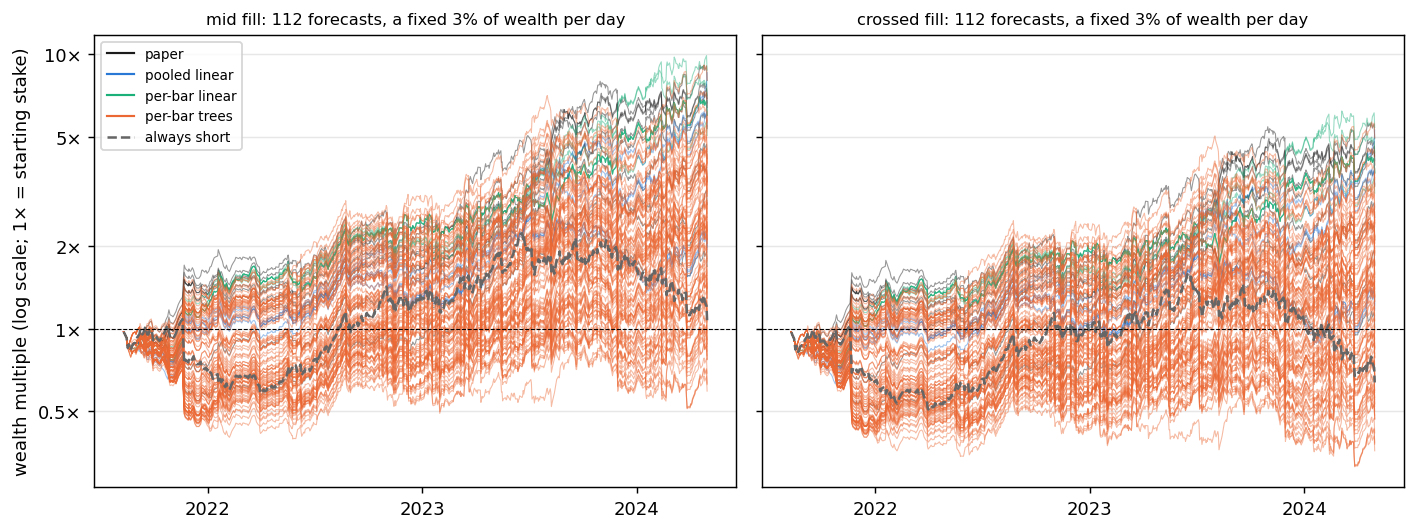
\includegraphics[width=\linewidth]{../results/close_compounding/wealth_modelset.png}
% % 2026-10-15 (notation pass): parked -- dummy day index s -> u (s_t is the signal); mid/crossed fill
% % \caption{Compounding at a fixed fraction: wealth $W_t = \prod_{s\le t}(1 + f q_s R_s)$ with $f =
% % \rhappCompF\,\%$ of wealth staked as straddle premium every day, $q_s = \pm 1$ the forecast's $\sign(s)$ position and
% % $R_s$ the straddle's return, for each of the \rhappModelSetN{} forecasts of the model set, mid fill (left) and crossed
% % fill (right), log scale; dashed: always short.}
% \caption{Compounded wealth at a fixed fraction. The figure plots $W_t = \prod_{u \le t}(1 + f\,q_u R_u)$, with
% $f = \rhappCompF\%$ of wealth committed as straddle premium each trading day, $q_u = \sign(s_u) = \pm 1$ the
% position of the sign strategy and $R_u$ the return on the straddle premium, for each of the \rhappModelSetN{}
% forecasts of the model set, at mid-quotes (left) and at quoted bid--ask prices (right), log scale; dashed: always
% short.}
% \label{fig:rh_app_wealth}
% \end{figure}

\clearpage

% =====================================================================================================================
% A4. The per-bar MinGRU's all-features diagnosis by day class. Sources: the walks' scores.csv (ql_month_end,
% ql_extreme_inputs, ql_other), the classes in wd_enc_study/day_class.csv; the walk of record's gap is asserted against
% results/puffer_forecast_2026-10-12/af_diagnosis/gap_by_dayclass.csv.
% =====================================================================================================================

\begin{table}[htbp]
\centering
\small
\begin{threeparttable}
% 2026-10-15 (notation pass): parked -- code jargon (all-features, walk); finance-journal first sentence
% \caption{Where the all-features MinGRU loses: QLIKE by day class, per walk.}
% 2026-10-15 (table legibility): short caption, details in the notes; notes cut to about five sentences, method
% details referred to Methods. The pre-notation-pass caption and notes are parked in the comments here.
\caption{MinGRU accuracy by type of trading day}
\label{tab:rh_app_mingru_dayclass}
% AUTO-GENERATED by writeup/make_rehaul_appendix.py -- do not edit.
% Source: results/puffer_forecast_2026-10-12/{wd_enc_study, lin_study, ridge_init_study, qlike_study}/scores.csv (ql_month_end, ql_extreme_inputs, ql_other); day classes wd_enc_study/day_class.csv; the walk of record's gap asserted against af_diagnosis/gap_by_dayclass.csv
\begin{tabular}{@{}l*{4}{r}@{}}
\toprule
 & Month-ends & Extreme inputs & Other days & All days \\
Walk & ($n = 43$) & ($n = 60$) & ($n = 763$) & ($n = 866$) \\
\midrule
\multicolumn{5}{@{}l}{\emph{QLIKE, HAR + calendar}} \\
\quad (1) Walk of record & 0.1478 & 0.1328 & 0.0949 & 0.1002 \\
\quad (2) Exogenous decay (B) & 0.1534 & 0.1091 & 0.0952 & 0.0990 \\
\quad (3) Linear shortcut (B) & 0.1444 & 0.0902 & 0.0951 & 0.0972 \\
\quad (4) Ridge start (b), MSE & 0.1420 & 0.1136 & 0.0951 & 0.0987 \\
\quad (5) (4), QLIKE selection & 0.1350 & 0.1062 & 0.0936 & 0.0966 \\
\quad (6) (4), QLIKE training & 0.1271 & 0.1190 & 0.0953 & 0.0985 \\
\quad Elastic net & 0.1542 & 0.1163 & 0.0895 & 0.0946 \\
\quad Ridge & 0.1542 & 0.1163 & 0.0896 & 0.0946 \\
\addlinespace
\multicolumn{5}{@{}l}{\emph{QLIKE, all features}} \\
\quad (1) Walk of record & 0.2323 & 0.2165 & 0.0927 & 0.1082 \\
\quad (2) Exogenous decay (B) & 0.1948 & 0.1735 & 0.0950 & 0.1054 \\
\quad (3) Linear shortcut (B) & 0.1399 & 0.3316 & 0.0992 & 0.1174 \\
\quad (4) Ridge start (b), MSE & 0.1586 & 0.1818 & 0.0927 & 0.1021 \\
\quad (5) (4), QLIKE selection & 0.1274 & 0.1362 & 0.0934 & 0.0980 \\
\quad (6) (4), QLIKE training & 0.1198 & 0.1527 & 0.0888 & 0.0948 \\
\quad Elastic net & 0.1376 & 0.1764 & 0.0853 & 0.0942 \\
\quad Ridge & 0.1361 & 0.1852 & 0.0865 & 0.0958 \\
\addlinespace
\multicolumn{5}{@{}l}{\emph{All features minus HAR + calendar}} \\
\quad (1) Walk of record & 0.0845 & 0.0837 & \ensuremath{-}0.0023 & 0.0080 \\
\quad (2) Exogenous decay (B) & 0.0413 & 0.0644 & \ensuremath{-}0.0002 & 0.0063 \\
\quad (3) Linear shortcut (B) & \ensuremath{-}0.0045 & 0.2414 & 0.0042 & 0.0202 \\
\quad (4) Ridge start (b), MSE & 0.0166 & 0.0682 & \ensuremath{-}0.0024 & 0.0034 \\
\quad (5) (4), QLIKE selection & \ensuremath{-}0.0076 & 0.0299 & \ensuremath{-}0.0003 & 0.0015 \\
\quad (6) (4), QLIKE training & \ensuremath{-}0.0074 & 0.0337 & \ensuremath{-}0.0065 & \ensuremath{-}0.0037 \\
\quad Elastic net & \ensuremath{-}0.0166 & 0.0601 & \ensuremath{-}0.0042 & \ensuremath{-}0.0004 \\
\quad Ridge & \ensuremath{-}0.0181 & 0.0689 & \ensuremath{-}0.0031 & 0.0011 \\
\bottomrule
\end{tabular}

\begin{tablenotes}[flushleft]
\footnotesize
% 2026-10-15 (notation pass): parked -- code jargon (walks, sessions, is_month_end, inputs, walk of record, gap)
% \item[] \emph{Notes:} walks (1)--(6) of Table~\ref{tab:rh_app_mingru_dev}. Month-ends: the sessions flagged \texttt{is\_month\_end}
% (\rhappNmonthEndExtreme{} of them also have extreme inputs). Extreme inputs: at least \rhappExtremeCols{} kept
% columns beyond their training-window maximum, month-ends excluded. The classes partition the \rhappNdays{} days, so
% the day-weighted mean of the three class columns is the overall QLIKE. Of the walk of record's summed daily gap
% between its all-features and HAR + calendar forecasts, extreme-input days carry \rhappGapShareExtreme\,\%, month-ends
% \rhappGapShareMonthEnd\,\% and the other days \rhappGapShareOther\,\%.
\item[] \textit{Notes:} Mean QLIKE of specifications (1)--(6) of Table~\ref{tab:rh_app_mingru_dev} by day type.
Month-ends: the last trading day of each calendar month (\rhappNmonthEndExtreme{} of them also have extreme predictor
values); extreme predictor values: at least \rhappExtremeCols{} retained columns above their estimation-window
maximum, month-ends excluded. The three day types partition the \rhappNdays{} trading days of the out-of-sample
period, so their day-weighted mean equals the overall mean QLIKE. Of the summed daily QLIKE loss differential of
specification (1) between the full predictor set and the HAR benchmark, days with extreme predictor values account
for \rhappGapShareExtreme\%, month-ends for \rhappGapShareMonthEnd\% and the other days for \rhappGapShareOther\%.
\end{tablenotes}
\end{threeparttable}
\end{table}

\clearpage

% 2026-10-15: the feature dictionary (47 series), moved here from 04_features_floats.tex (Appendix A).
% generated by writeup/make_rehaul_data_methods.py -- do not edit by hand; change the generator and re-run.
\providecommand{\rdmL}{\raggedright\let\\\tabularnewline}
\providecommand{\rdmR}{\raggedleft\let\\\tabularnewline}

\begingroup
\footnotesize
\setlength{\tabcolsep}{4pt}
\setlength{\LTcapwidth}{\textwidth}
\begin{longtable}{@{}p{\dimexpr(\textwidth-10\tabcolsep)*220/1000\relax}p{\dimexpr(\textwidth-10\tabcolsep)*300/1000\relax}p{\dimexpr(\textwidth-10\tabcolsep)*190/1000\relax}p{\dimexpr(\textwidth-10\tabcolsep)*130/1000\relax}p{\dimexpr(\textwidth-10\tabcolsep)*80/1000\relax}p{\dimexpr(\textwidth-10\tabcolsep)*80/1000\relax}@{}}
\caption{Feature dictionary: the 47 exogenous series.}\label{tab:rh_dm_dictionary}\\
\toprule
\rdmL Series & \rdmL Raw statistic & \rdmL Source file & \rdmL Transform & \rdmL Diurnal & \rdmL Active \\
\midrule
\endfirsthead
\multicolumn{6}{@{}l}{\textit{Table \ref{tab:rh_dm_dictionary} (continued)}}\\
\toprule
\rdmL Series & \rdmL Raw statistic & \rdmL Source file & \rdmL Transform & \rdmL Diurnal & \rdmL Active \\
\midrule
\endhead
\midrule
\multicolumn{6}{r@{}}{\textit{continued on the next page}}\\
\endfoot
\bottomrule
\multicolumn{6}{@{}p{\textwidth}@{}}{\rdmL\rule{0pt}{2.5ex}\textit{Notes:} One row per exogenous series, by bucket. Derived programmatically: the bucket from \texttt{src/data/loading.py}; the transform from the branch \texttt{apply\_semantic\_transform} takes for the column name and sign (\texttt{src/features/transforms/target.py}); the diurnal adjustment and the asinh routing from \texttt{robust\_transform} run on the forward-filled panel; the activity flag from the executor's mode-inflation rule (modal value on at least 20\,\% of rows), checked against the design's \texttt{\_active} columns. Diurnal: mean, divided by the trailing same-slot mean (20 observations, at least 5, lagged one bar); s.d., divided by the trailing same-slot standard deviation (floored); both banded to $[0.5, 2]$ times the slot's trailing 250-observation median; none: the VIX family, sentiment and the FOMC flags. asinh: a signed series whose s.d.\ divisor sits on its floor on at least 50\,\% of rows skips the division and takes $\operatorname{asinh}(x/s_t)$, $s_t$ a causal EWMA of $|x|$. $x$: no transform (signed series and \texttt{sumabsret}); a series counts as signed if it has any negative value (\texttt{spread\_vwstock} is signed by 1 negative print, 2018-11-12 11:00, and so takes $x$ and s.d.\ where its EW twin takes $\log x$ and mean). After the transform every series is winsorised at rolling 240-bar 1\,/\,99\,\% bounds, set to its median where unobserved, laddered and scaled. Modes of the active series (share of rows): \texttt{numobs} 30 (72\%); \texttt{voldemand\_\allowbreak{}spx\_\allowbreak{}open\_\allowbreak{}and\_\allowbreak{}close} 0 (59\%); \texttt{voldemand\_\allowbreak{}spx\_\allowbreak{}open\_\allowbreak{}only} 0 (60\%); \texttt{voldemand\_\allowbreak{}all\_\allowbreak{}open\_\allowbreak{}and\_\allowbreak{}close} 0 (59\%); \texttt{voldemand\_\allowbreak{}all\_\allowbreak{}open\_\allowbreak{}only} 0 (60\%); \texttt{fomc\_\allowbreak{}release} 0 (98\%); \texttt{fomc\_\allowbreak{}day} 0 (95\%).}\\
\endlastfoot
\multicolumn{6}{@{}l}{\textit{ES return moments (7)}} \\
\rdmL \texttt{sumret} & \rdmL bar return $\sum r$ & \rdmL \texttt{core\_\allowbreak{}stats} & \rdmL $x$ & \rdmL s.d. & \rdmL no \\
\rdmL \texttt{sumabsret} & \rdmL $\sum |r|$ & \rdmL \texttt{core\_\allowbreak{}stats} & \rdmL $x$ & \rdmL mean & \rdmL no \\
\rdmL \texttt{sumret3} & \rdmL $\sum r^3$ & \rdmL \texttt{core\_\allowbreak{}stats} & \rdmL $x^{1/3}$ & \rdmL s.d. & \rdmL no \\
\rdmL \texttt{sumret4} & \rdmL $\sum r^4$ & \rdmL \texttt{core\_\allowbreak{}stats} & \rdmL $\pm|x|^{1/4}$ & \rdmL mean & \rdmL no \\
\rdmL \texttt{sumpret2} & \rdmL upside semivariance $\sum r^2 \mathbf{1}\{r>0\}$ & \rdmL \texttt{core\_\allowbreak{}stats} & \rdmL $\sqrt{x}$ & \rdmL mean & \rdmL no \\
\rdmL \texttt{sumbipow} & \rdmL bipower variation & \rdmL \texttt{core\_\allowbreak{}stats} & \rdmL $\sqrt{x}$ & \rdmL mean & \rdmL no \\
\rdmL \texttt{sumautocov} & \rdmL first-order autocovariance $\sum r_i r_{i-1}$ & \rdmL \texttt{core\_\allowbreak{}stats} & \rdmL $\pm\sqrt{|x|}$ & \rdmL s.d. & \rdmL no \\
\addlinespace
\multicolumn{6}{@{}l}{\textit{Liquidity (14)}} \\
\rdmL \texttt{sumvolume} & \rdmL contract volume & \rdmL \texttt{core\_\allowbreak{}stats} & \rdmL $\log x$ & \rdmL mean & \rdmL no \\
\rdmL \texttt{numobs} & \rdmL 1-min returns in the bar ($\le 30$) & \rdmL \texttt{core\_\allowbreak{}stats} & \rdmL $\log x$ & \rdmL mean & \rdmL yes \\
\rdmL \texttt{turnover\_\allowbreak{}ewstock} & \rdmL turnover & \rdmL \texttt{ewstock\_\allowbreak{}stats} & \rdmL $\sqrt{x}$ & \rdmL mean & \rdmL no \\
\rdmL \texttt{buyturnover\_\allowbreak{}ewstock} & \rdmL buyer-initiated turnover & \rdmL \texttt{ewstock\_\allowbreak{}stats} & \rdmL $\sqrt{x}$ & \rdmL mean & \rdmL no \\
\rdmL \texttt{sellturnover\_\allowbreak{}ewstock} & \rdmL seller-initiated turnover & \rdmL \texttt{ewstock\_\allowbreak{}stats} & \rdmL $\sqrt{x}$ & \rdmL mean & \rdmL no \\
\rdmL \texttt{effspread\_\allowbreak{}ewstock} & \rdmL effective spread & \rdmL \texttt{ewstock\_\allowbreak{}stats} & \rdmL $\sqrt{x}$ & \rdmL mean & \rdmL no \\
\rdmL \texttt{spread\_\allowbreak{}ewstock} & \rdmL quoted spread & \rdmL \texttt{ewstock\_\allowbreak{}stats} & \rdmL $\log x$ & \rdmL mean & \rdmL no \\
\rdmL \texttt{turnover\_\allowbreak{}vwstock} & \rdmL turnover & \rdmL \texttt{vwstock\_\allowbreak{}stats} & \rdmL $\sqrt{x}$ & \rdmL mean & \rdmL no \\
\rdmL \texttt{buyturnover\_\allowbreak{}vwstock} & \rdmL buyer-initiated turnover & \rdmL \texttt{vwstock\_\allowbreak{}stats} & \rdmL $\sqrt{x}$ & \rdmL mean & \rdmL no \\
\rdmL \texttt{sellturnover\_\allowbreak{}vwstock} & \rdmL seller-initiated turnover & \rdmL \texttt{vwstock\_\allowbreak{}stats} & \rdmL $\sqrt{x}$ & \rdmL mean & \rdmL no \\
\rdmL \texttt{effspread\_\allowbreak{}vwstock} & \rdmL effective spread & \rdmL \texttt{vwstock\_\allowbreak{}stats} & \rdmL $\sqrt{x}$ & \rdmL mean & \rdmL no \\
\rdmL \texttt{spread\_\allowbreak{}vwstock} & \rdmL quoted spread & \rdmL \texttt{vwstock\_\allowbreak{}stats} & \rdmL $x$ & \rdmL s.d. & \rdmL no \\
\rdmL \texttt{ofi\_\allowbreak{}ewstock} & \rdmL order-flow imbalance $(b-s)/(b+s)$ of turnover & \rdmL \texttt{ewstock\_\allowbreak{}stats} (derived) & \rdmL $x$ & \rdmL s.d. & \rdmL no \\
\rdmL \texttt{ofi\_\allowbreak{}vwstock} & \rdmL order-flow imbalance $(b-s)/(b+s)$ of turnover & \rdmL \texttt{vwstock\_\allowbreak{}stats} (derived) & \rdmL $x$ & \rdmL s.d. & \rdmL no \\
\addlinespace
\multicolumn{6}{@{}l}{\textit{Market, equal-weighted (6)}} \\
\rdmL \texttt{sumret2\_\allowbreak{}ewstock} & \rdmL realized variance $\sum r^2$ & \rdmL \texttt{ewstock\_\allowbreak{}stats} & \rdmL $\sqrt{x}$ & \rdmL mean & \rdmL no \\
\rdmL \texttt{sumret3\_\allowbreak{}ewstock} & \rdmL $\sum r^3$ & \rdmL \texttt{ewstock\_\allowbreak{}stats} & \rdmL $x^{1/3}$ & \rdmL s.d. & \rdmL no \\
\rdmL \texttt{sumret4\_\allowbreak{}ewstock} & \rdmL $\sum r^4$ & \rdmL \texttt{ewstock\_\allowbreak{}stats} & \rdmL $\pm|x|^{1/4}$ & \rdmL mean & \rdmL no \\
\rdmL \texttt{sumabsret\_\allowbreak{}ewstock} & \rdmL $\sum |r|$ & \rdmL \texttt{ewstock\_\allowbreak{}stats} & \rdmL $x$ & \rdmL mean & \rdmL no \\
\rdmL \texttt{sumbipow\_\allowbreak{}ewstock} & \rdmL bipower variation & \rdmL \texttt{ewstock\_\allowbreak{}stats} & \rdmL $\sqrt{x}$ & \rdmL mean & \rdmL no \\
\rdmL \texttt{sumpret2\_\allowbreak{}ewstock} & \rdmL upside semivariance $\sum r^2 \mathbf{1}\{r>0\}$ & \rdmL \texttt{ewstock\_\allowbreak{}stats} & \rdmL $\sqrt{x}$ & \rdmL mean & \rdmL no \\
\addlinespace
\multicolumn{6}{@{}l}{\textit{Market, value-weighted (6)}} \\
\rdmL \texttt{sumret2\_\allowbreak{}vwstock} & \rdmL realized variance $\sum r^2$ & \rdmL \texttt{vwstock\_\allowbreak{}stats} & \rdmL $\sqrt{x}$ & \rdmL mean & \rdmL no \\
\rdmL \texttt{sumret3\_\allowbreak{}vwstock} & \rdmL $\sum r^3$ & \rdmL \texttt{vwstock\_\allowbreak{}stats} & \rdmL $x^{1/3}$ & \rdmL s.d. & \rdmL no \\
\rdmL \texttt{sumret4\_\allowbreak{}vwstock} & \rdmL $\sum r^4$ & \rdmL \texttt{vwstock\_\allowbreak{}stats} & \rdmL $\pm|x|^{1/4}$ & \rdmL mean & \rdmL no \\
\rdmL \texttt{sumabsret\_\allowbreak{}vwstock} & \rdmL $\sum |r|$ & \rdmL \texttt{vwstock\_\allowbreak{}stats} & \rdmL $x$ & \rdmL mean & \rdmL no \\
\rdmL \texttt{sumbipow\_\allowbreak{}vwstock} & \rdmL bipower variation & \rdmL \texttt{vwstock\_\allowbreak{}stats} & \rdmL $\sqrt{x}$ & \rdmL mean & \rdmL no \\
\rdmL \texttt{sumpret2\_\allowbreak{}vwstock} & \rdmL upside semivariance $\sum r^2 \mathbf{1}\{r>0\}$ & \rdmL \texttt{vwstock\_\allowbreak{}stats} & \rdmL $\sqrt{x}$ & \rdmL mean & \rdmL no \\
\addlinespace
\multicolumn{6}{@{}l}{\textit{Sentiment (3)}} \\
\rdmL \texttt{stocktwits\_\allowbreak{}attention} & \rdmL message volume (attention) & \rdmL \texttt{spy\_\allowbreak{}and\_\allowbreak{}sentiment} & \rdmL $\log x$ & \rdmL mean & \rdmL no \\
\rdmL \texttt{stocktwits\_\allowbreak{}sentiment} & \rdmL net sentiment score & \rdmL \texttt{spy\_\allowbreak{}and\_\allowbreak{}sentiment} & \rdmL $x$ & \rdmL none & \rdmL no \\
\rdmL \texttt{stocktwits\_\allowbreak{}sentcount} & \rdmL messages with a sentiment tag & \rdmL \texttt{spy\_\allowbreak{}and\_\allowbreak{}sentiment} & \rdmL $\log x$ & \rdmL mean & \rdmL no \\
\addlinespace
\multicolumn{6}{@{}l}{\textit{Implied volatility (3)}} \\
\rdmL \texttt{vix} & \rdmL VIX level & \rdmL \texttt{vix\_\allowbreak{}and\_\allowbreak{}voldemand} & \rdmL $\log x$ & \rdmL none & \rdmL no \\
\rdmL \texttt{vvix} & \rdmL VVIX level & \rdmL \texttt{vix\_\allowbreak{}and\_\allowbreak{}voldemand} & \rdmL $\log x$ & \rdmL none & \rdmL no \\
\rdmL \texttt{vix3m} & \rdmL VIX3M level & \rdmL \texttt{vix\_\allowbreak{}and\_\allowbreak{}voldemand} & \rdmL $\log x$ & \rdmL none & \rdmL no \\
\addlinespace
\multicolumn{6}{@{}l}{\textit{Volatility demand (4)}} \\
\rdmL \texttt{voldemand\_\allowbreak{}spx\_\allowbreak{}open\_\allowbreak{}and\_\allowbreak{}close} & \rdmL SPX options, opening and closing & \rdmL \texttt{vix\_\allowbreak{}and\_\allowbreak{}voldemand} & \rdmL $\operatorname{asinh}(x/s_t)$ & \rdmL none & \rdmL yes \\
\rdmL \texttt{voldemand\_\allowbreak{}spx\_\allowbreak{}open\_\allowbreak{}only} & \rdmL SPX options, opening only & \rdmL \texttt{vix\_\allowbreak{}and\_\allowbreak{}voldemand} & \rdmL $\operatorname{asinh}(x/s_t)$ & \rdmL none & \rdmL yes \\
\rdmL \texttt{voldemand\_\allowbreak{}all\_\allowbreak{}open\_\allowbreak{}and\_\allowbreak{}close} & \rdmL all options, opening and closing & \rdmL \texttt{vix\_\allowbreak{}and\_\allowbreak{}voldemand} & \rdmL $\operatorname{asinh}(x/s_t)$ & \rdmL none & \rdmL yes \\
\rdmL \texttt{voldemand\_\allowbreak{}all\_\allowbreak{}open\_\allowbreak{}only} & \rdmL all options, opening only & \rdmL \texttt{vix\_\allowbreak{}and\_\allowbreak{}voldemand} & \rdmL $\operatorname{asinh}(x/s_t)$ & \rdmL none & \rdmL yes \\
\addlinespace
\multicolumn{6}{@{}l}{\textit{FOMC calendar (4)}} \\
\rdmL \texttt{fomc\_\allowbreak{}release} & \rdmL 1 on the 14:30 statement bar & \rdmL \texttt{releases} (derived) & \rdmL $\log x$ & \rdmL none & \rdmL yes \\
\rdmL \texttt{fomc\_\allowbreak{}day} & \rdmL 1 on statement days & \rdmL \texttt{releases} (derived) & \rdmL $\log x$ & \rdmL none & \rdmL yes \\
\rdmL \texttt{fomc\_\allowbreak{}until\_\allowbreak{}inv} & \rdmL $1/(1+{}$bars to next statement$)$ & \rdmL \texttt{releases} (derived) & \rdmL $\log x$ & \rdmL none & \rdmL no \\
\rdmL \texttt{fomc\_\allowbreak{}since\_\allowbreak{}inv} & \rdmL $1/(1+{}$bars since last$)$ & \rdmL \texttt{releases} (derived) & \rdmL $\log x$ & \rdmL none & \rdmL no \\
\end{longtable}
\endgroup

